\documentclass[letter, 12pt]{article}
\usepackage[utf8]{inputenc}
\usepackage{graphicx} % Allows you to insert figures
\usepackage{amsmath} % Allows you to do equations
\usepackage{hyperref}
\usepackage{fancyhdr} % Formats the header
\usepackage{geometry} % Formats the paper size, orientation, and margins
\usepackage[english]{babel}
\usepackage{csquotes}
\renewcommand*{\nameyeardelim}{\addcomma\space} % Adds comma in in-text citations
\linespread{1.25} % About 1.5 spacing in Word
\setlength{\parindent}{0pt} % No paragraph indents
\setlength{\parskip}{1em} % Paragraphs separated by one line
\renewcommand{\headrulewidth}{0pt} % Removes line in header
\geometry{letterpaper, portrait, margin=1in}
\setlength{\headheight}{14.49998pt}

\begin{document}
\begin{titlepage}
   \begin{center}
        \vspace*{2cm}

        \Huge{OVAL: Online Video Compression using Autoencoder Learning}

        \vspace{0.5cm}
        \LARGE{Project Proposal}
            
        \vspace{3 cm}
        \Large{Project Group 27} \\
        \Large{Word Count: 1393}
       
        \vspace{0.25cm}
        \large{Isidor Kaplan (1005904005) \\
        Adam Glustein (1006068425) \\
        Ryan Ghosh (1006418627) \\
        Khantil Desai (1006155161)}
       
        \vspace{3 cm}
        \Large{Feb. 9, 2022}
        
        \vspace{0.25 cm}
        \large{APS360 - Applied Fundamentals of Machine Learning, Winter 2022}
       

       \vfill
    \end{center}
\end{titlepage}

\setcounter{page}{2}
\pagestyle{fancy}
\fancyhf{}
\rhead{\thepage}
\lhead{OVAL: Online Video Compression using Autoencoder Learning}

\section{Introduction}

Real-time video conferencing has become increasingly important with the catalyst of the COVID-19 pandemic. As video data is continuously generated, it must be compressed and decompressed with lossy reconstruction. Finding efficient compressions is a task well-suited to artificial neural networks, especially autoencoders, since they reduce inputs into smaller latent-space representations. Existing video compression methods are either algorithmic or based on offline training, and therefore cannot adapt to individual video streams. OVAL aims to create a novel online learning model for video compression which finds efficient video encodings in real-time. By reducing the size of in-conference transmissions, OVAL will mitigate lag and other undesirable qualities. 

\section{Visualization of OVAL}


\begin{figure}[h] % h - Place the float here, i.e., approximately at the same point it occurs in the source text (however, not exactly at the spot)
\centering
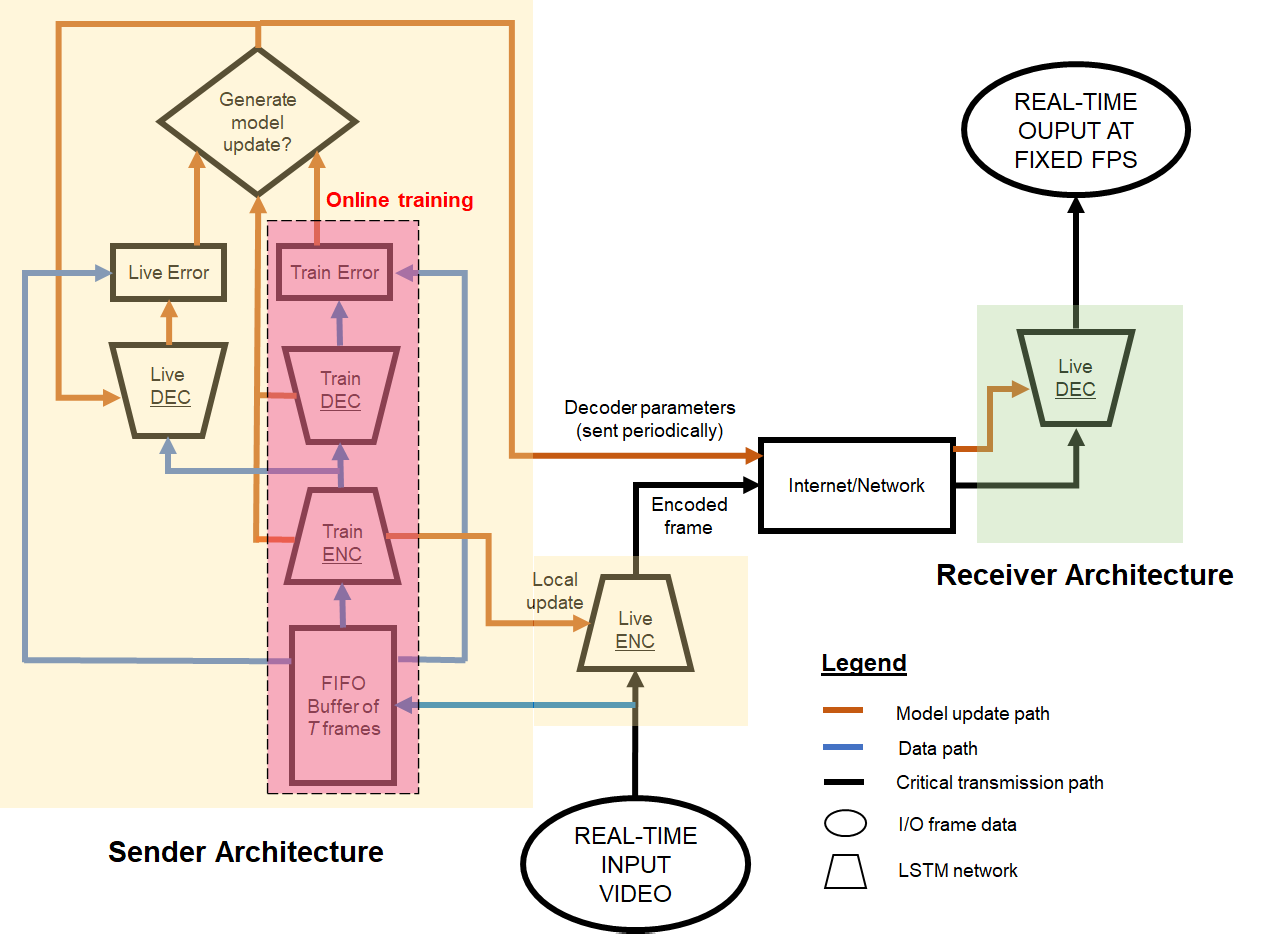
\includegraphics[width=18cm]{isidor_arch_diag.png}
\caption{The high-level architecture of the OVAL model, allowing for concurrent online learning and encoding.}
\label{fig:bigarch}
\end{figure}

In the \textit{critical path }(\textbf{Figure \ref{fig:bigarch}}), video frames are encoded and sent to the receiver. The receiver decodes the data using parameters which are periodically updated by the sender. As the sender encodes frames, the model performs unsupervised learning using the input video data. In an isolated pipeline, data moves through a FIFO buffer to a training-stage autoencoder. The training error is compared to the live error and OVAL decides whether to update the receiver with new model parameters. The dynamic update policy allows large live errors to be corrected promptly while small errors need to be corrected infrequently.

The sender's neural network autoencoders (\textbf{Figure \ref{fig:arch}}) are used separately for training and live encoding, which is necessary for online learning. The receiver's decoder does not need to be identical to the sender's if a small live error is preserved during transmission. Thus, having two separate live decoders reduces the transfer of decoder parameters between sender and receiver. 

\clearpage
\section{Background and Related Work}

Autoencoders have previously been used for video compression and summarization, with most approaches using offline learning and offline encoding (offline-offline). A recent paper [1] used autoencoders for video compression with offline training but online encoding. Using a fixed recurrent neural network, the pre-trained model was able to encode videos in real-time. Upon validation, the model achieved a state-of-the-art MS-SSIM similarity index which outperformed existing offline-offline models and traditional codecs. 

Another recent paper [2] used online training with offline encoding. Again using an autoencoder neural network, the model learned frame-by-frame representations for video summarization. However, when tested on new data, the model required the entire new video before it could encode a summarization. Their model achieved state-of-the-art performance for summarizing object motion in video. The network architecture consisted of initial convolution layers for feature extraction and three series LSTM encoding layers.

\section{Design Considerations}

\subsection{Data Processing and Training}

Autoencoders will be pre-trained in an offline learning phase and continuously improve in an online learning phase.

\begin{figure}[h] % h - Place the float here, i.e., approximately at the same point it occurs in the source text (however, not exactly at the spot)
\centering
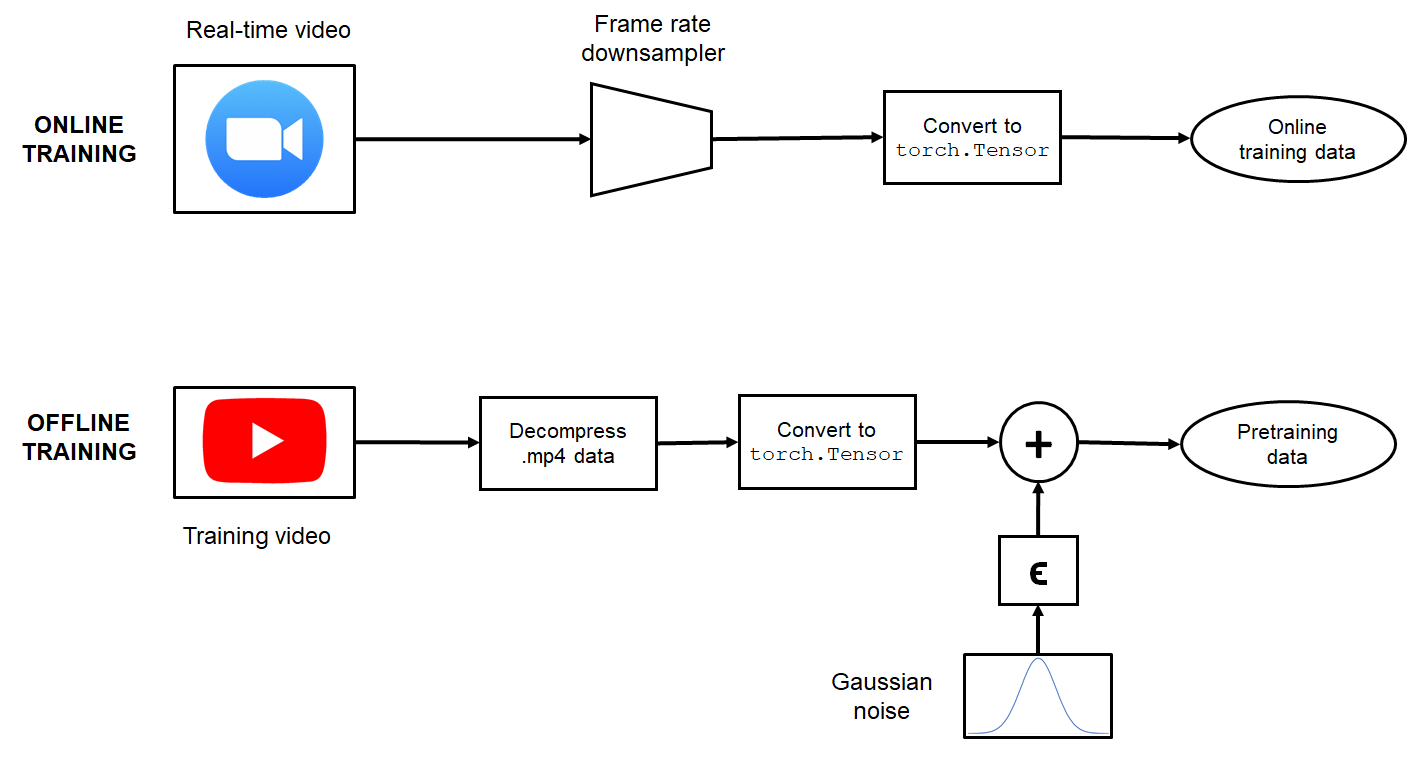
\includegraphics[width=16cm]{data_pipeline.png}
\caption{Offline and online data processing for model training.}
\label{fig:data}
\end{figure}


\subsubsection{Offline Data Pipeline}

Training data will be YouTube talk show clips from CBC, BBC, CNN and Fox News [3,4]. Each clip will be 5-10 minutes long and focus on a single individual speaking to a camera. These videos are similar to video conferencing and short enough to store in RAM memory. There are no openly available video conferencing datasets.

In\textbf{ Figure \ref{fig:data}}, YouTube videos are downloaded as MP4 files and converted to tensors. Gaussian noise is added with a variable gain $\epsilon$ to avoid overfitting before passing input to the autoencoder.

\subsubsection{Online Data Pipeline}

Online training data will come from the real-time video feed being encoded. If data is entering the queue in \textbf{Figure \ref{fig:bigarch}} faster than it is being processed, we downsample the training video to ensure training data does not fall behind the live feed.

\subsection{Architecture}

Each node or user has two autoencoders; one for training more efficient compression and one for live encoding/decoding. The autoencoders each contain two LSTMs, a form of recurrent neural network (RNN) suited for sequential data. LSTMs are preferable to standard RNNs since they can remember invariant information from prior frames to allow for smaller encodings. We also apply convolutional layers for feature extraction and resampling data. \textbf{Figure \ref{fig:arch}} shows the detailed architecture for the autoencoder. 

\begin{figure}[h!] % h - Place the float here, i.e., approximately at the same point it occurs in the source text (however, not exactly at the spot)
\centering
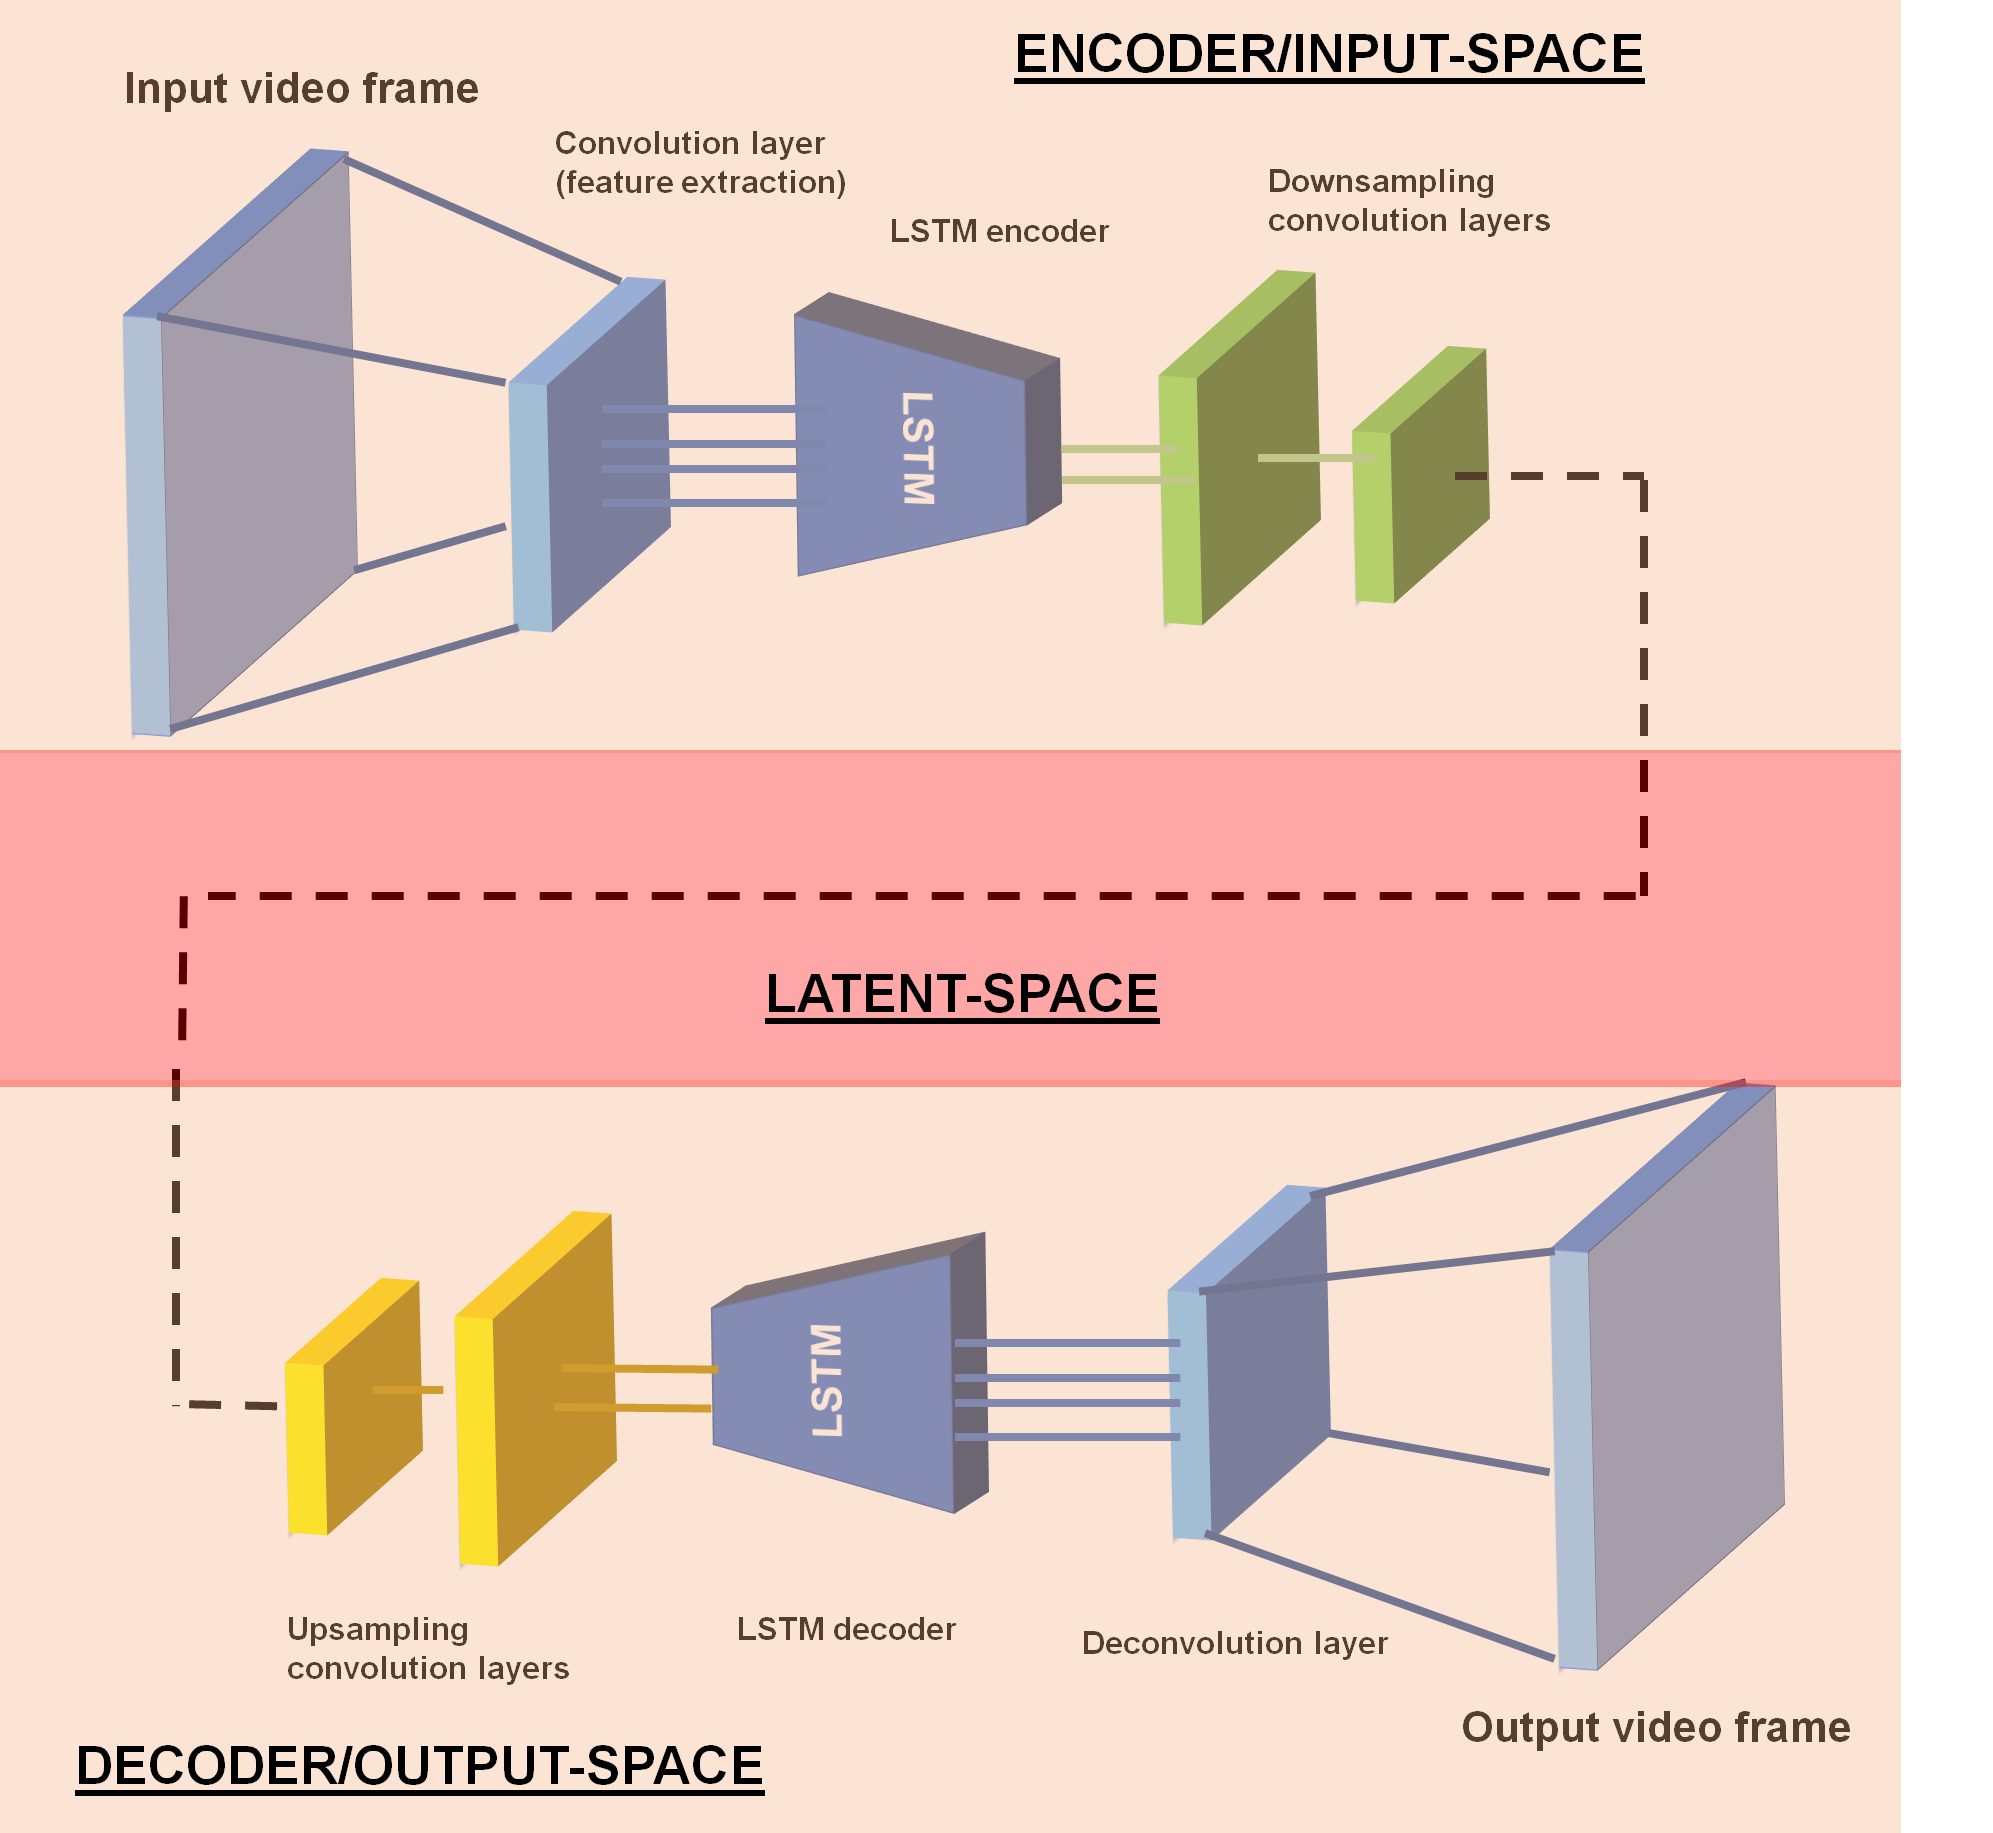
\includegraphics[width=16cm]{architecture.png}
\caption{The OVAL autoencoder architecture, designed to convert input frames into compact latent-space representations which can be decoded by a receiver. }
\label{fig:arch}
\end{figure}

In Figure \ref{fig:arch}, the sampling convolution layers are symmetric in shape between the input-space and output-space, which allows for variable encoding sizes. If high loss is detected in the network, then larger encodings can be used from earlier convolution layers. If loss is small, then encodings can become more efficient by using later convolution layers. All encoding levels are pre-trained offline. During online learning, we use an \textit{epsilon-greedy} strategy for choosing the encoding level to balance exploration and exploitation.

Since the primary application of OVAL is video conferencing, the architecture must be able to scale efficiently. OVAL can use federated learning to optimize training efficiency. Each node shares parameters with a global model that fits to all users on the call. Then, the individual nodes incorporate the global parameters in their next training iteration to avoid decoherence. This ensures the nodes learn concurrently without input-data transfer over the network (\textbf{Figure \ref{fig:fed}}).

\begin{figure}[h!] % h - Place the float here, i.e., approximately at the same point it occurs in the source text (however, not exactly at the spot)
\centering
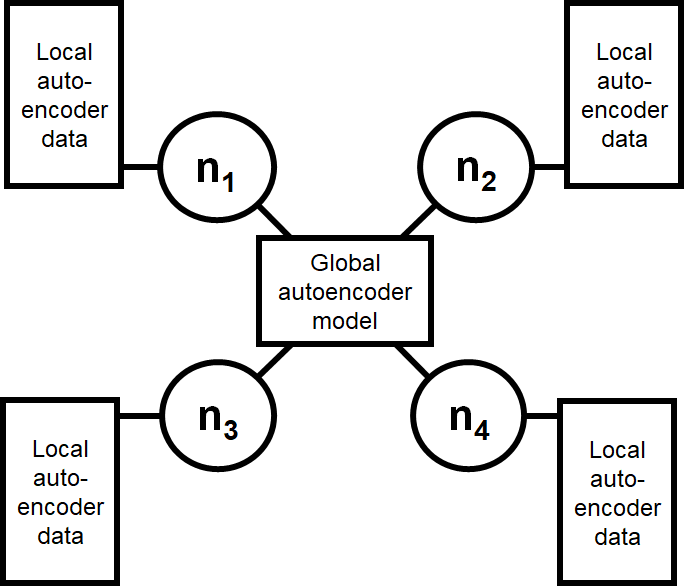
\includegraphics[width=12cm]{federated.png}
\caption{Federated learning network using OVAL encoding on a video conference with four user nodes, $n_1$ to $n_4$. Each node is able to broadcast encoder parameters to a centralized global server for all users on the call.}
\label{fig:fed}
\end{figure}


\subsection{Baseline Model}

Algorithmic video codecs are still the primary method of video compression, with the most common standard being MPEG-4. MPEG-4 uses mathematical transforms to reduce encoding sizes. Identical video data will be provided to OVAL and an MPEG-4 encoder and comparisons can be made based on compression ratio, video similarity index (MS-SSIM) and qualitative viewing. 

\subsection{Ethical Considerations}

Equitable representation of video users is crucial for fair training. Training videos will contain people of different ethnicities to ensure compression does not favor a biased demographic. OVAL will also be trained online using hardware of varying quality to ensure we do not overfit to expensive devices. 
 
An ethical issue in OVAL is data privacy, especially using federated learning (Section 4.2). Autoencoder parameters could be exploited to uncover sensitive information about a video conference. We will reset all autoencoders for every new conference to make past data inaccessible. In-conference encoder data will also be protected with end-to-end encryption.
\section{Project Management}

\subsection{Project Plan}

Our team will meet weekly on Mondays at 9 pm to align our goals. We communicate over a Discord server with channels reserved for distinct topics. We use Git for version control and resolve merge conflicts by communicating with the conflicting members first. To organize workflow, we divided the project into five stages in \textbf{Table \ref{work}}.


\begin{table}[h!]\centering
   \begin{tabular}{ |p{7.5cm}|p{1.5cm}|p{2.5cm}|p{2.5cm}|  }
\hline
Task Name & Member & Estimated Time & Deadline \\
\hline
\multicolumn{3}{|c|}{\textbf{Stage 1: Idea Generation and Proposal}} & \textbf{Feb. 9} \\
\hline
Research survey & All & 3 hr/ea & Jan. 26 \\
Project idea & Isidor & 3 hr & Jan. 27 \\
Architecture design & Isidor & 3 hr & Jan. 27 \\
Formal proposal & Adam & 8 hr & Feb. 3 \\
\hline
\multicolumn{3}{|c|}{\textbf{Stage 2: Minimum Viable Product (MVP)}} & \textbf{Feb. 19}\\
\hline
Data processing code & Khantil & 8 hr & Feb. 4 \\
Full offline implementation & Ryan & 12 hr & Feb. 10 \\
Variable-length encoding & Ryan & 3 hr & Feb. 10 \\
Offline training code & Khantil & 8 hr & Feb. 12 \\
Online simulator code & Isidor & 3 hr & Feb. 12 \\
Integrating online/offline components & Isidor & 3 hr & Feb. 14 \\
Sender architecture code & Isidor & 5 hr & Feb. 17 \\
\hline
\multicolumn{3}{|c|}{\textbf{Stage 3: Proof-of-Concept (POC)}} & \textbf{Mar. 12} \\
\hline
Single-sender simulator code & Isidor & 7 hr & Feb. 20 \\
Hyperparameter tuning & Adam & 8 hr & Feb. 26 \\
Evaluation on sample videos & Ryan & 5 hr & Feb. 28 \\
Benchmark on full-scale dataset & Khantil & 8 hr & Mar. 4 \\
\hline
\multicolumn{3}{|c|}{\textbf{Stage 4: Federated Learning Extension}} & \textbf{Mar. 19}\\
\hline
Networking code for federated learning & Adam & 6 hr & Mar. 10 \\
Global autoencoder broadcast code & Ryan & 6 hr & Mar. 12 \\
Integrate complete federated model & Isidor & 7 hr & Mar. 15 \\
\hline
\multicolumn{3}{|c|}{\textbf{Stage 5: Presentation and Publication}} & \textbf{Apr. 5} \\
\hline
Final report  & Adam & 8 hr & Mar. 31 \\
Final presentation  & All & 10 hr & Mar. 31 \\
\hline

\end{tabular} 
\caption{Individual responsibilities at each project stage including internal deadlines.}
\label{work}
\end{table}


\subsection{Risk Register}

\begin{enumerate}
    \item \textbf{Project complexity     } The OVAL project is highly complex which creates the risk that we may not be able to finish by April. We manage this risk by including various \textit{cutoff points} in the project where remaining work is expected but not necessary. For example, the most basic cutoff point is building a single autoencoder for video data, which has been achieved in many papers.
    \item \textbf{Insufficient architecture     } A single LSTM encoder layer may be insufficient in compressing video data to meet benchmark performance. For example, the related work with online training [2] used three separate LSTM layers. To alleviate this risk, we will design all components using proper modularization. Thus, we can easily change the architecture without major changes to the codebase.
    \item \textbf{Fatal processing delay    }   Concurrent encoding and training may be unable to process high frame rate video. To alleviate this risk, we will downsample training frames if the model detects lag. Thus, a consistent rate of training data can be ingested regardless of the input frame rate.
    \item \textbf{Network congestion     } Since senders periodically send their decoders to receivers, a large number of concurrent users could produce overwhelming load on a computer network. To alleviate this risk, we will begin with a single sender-receiver to demonstrate OVAL's proof-of-concept. Then, if possible, we can extend the system to multi-agent use.
\end{enumerate}

\subsection{GitHub Link}

\textbf{\href{https://gitfront.io/r/IsidorJKaplan/66735f7a469e427f884c3c37717656a3ca7de0f5/OVAL/}{https://gitfront.io/r/IsidorJKaplan/.../OVAL/}}

\pagebreak

\section*{References}

[1]  A. Golinski, R. Pourreza, Y. Yang, S. Guillaume and S. Taco. ``Feedback Recurrent Autoencoder for Video Compression," Qualcomm AI Research, 2020. 

[2] Y. Zhang, X. Liang, D. Zhang, M. Tan, and E. P. Xing, ``Unsupervised object-level video summarization with online motion auto-encoder,” Pattern Recognition Letters, vol. 130, pp. 376–385, 2020. 

[3] “CNN,” YouTube. [Online]. Available: https://www.youtube.com/user/CNN. [Accessed: 03-Feb-2022]. 

[4] “BBC News,” YouTube. [Online]. Available: https://www.youtube.com/c/BBCNews. [Accessed: 03-Feb-2022]. 

\end{document}

